
\chapter{Physics}
\label{chap:physics}

\section{Electromagnetism}	%maybe exclude this section?

Electromagnetism is one of the four fundamental forces at the common level of energy. In all situations examined in this thesis (sw plasma, magnetosphere) it is by far the strongest force and the others can be neglected.\\

%Lorentz force law as the definition of E and B\\
%The electromagnetic force F on a test charge at a given point and time is a certain function of its charge q and velocity v, which can be parameterized by exactly two vectors E and B, in the functional form: (wiki)\\
The Lorentz force: $\textbf{F} = q (\textbf{E} + \textbf{v} \times \textbf{B})$\\

The Maxwell equations in differential notation:
\begin{align}
	\text{div}\,\textbf{B} &= 0\\
	\text{div}\,\textbf{D} &= \rho\\
	\text{rot}\,\textbf{H} &= \textbf{j} + \dot{\textbf{D}}\\
	\text{rot}\,\textbf{E} &= - \dot{\textbf{B}}
\end{align}
With the magnetic flux density \textbf{B} (aka magnetic field), the electric displacement field \textbf{D}, the charge density $\rho$, the magnetic field \textbf{H}, the electric field \textbf{E} and the current density \textbf{j}.\\
%note about B naming convention within this work as magnetic field strength% maybe put into beginning...


\section{Solar wind pressures}

The magnetic energy density $w_\text{mag}$ is also the magnetic pressure $p_\text{mag}$
\begin{align}
	w_\text{mag} &= p_\text{mag}\\
	&= \frac{B^2}{2 \mu_0}	\text{\,.}
\end{align}

dynamic pressure $p_\text{dyn} = \rho v^2$\\
thermal pressure $p_\text{therm} = n k_\text{B} T$\\
magnetic pressure $p_\text{mag} = B^2 / (2 \mu_0)$ (see above...)\\
ram pressure??\\
%VB1998p104


\section{Plasma beta}
\label{sec:plasma_beta}
In MHD the magnetic energy density behaves like an additional pressure that adds to the gas pressure of a plasma (Wikipedia; find alternative source...).

The ratio of the thermal pressure $p = n k_\text{B} T$ to the magnetic pressure $p_\text{mag} = \frac{B^2}{2 \mu_0}$ is called plasma beta
\begin{align}
	\beta &= \frac{p}{p_\text{mag}}\\
	&= \frac{2 \mu_0 n k_\text{B} T}{B^2}
\end{align}
with the number density $n$.\\
$\beta \ll 1$: ``cold'' plasma; magnetic field contains plasma (magnetic clouds)\\
$\beta \geq 1$: ``warm'' plasma; plasma keeps magnetic field

%aka proton beta
plasma beta see \citep[p.~50]{Kivelson1995}

typical $beta$-values for solar wind are in the range X--Y.\\

% Plasma beta:\\
% near-sun β << 1:\\
% far-sun β ≥ 1:\\
% β = p /pkin mag\\
% plasma follows magnetic field\\
% magnetic field is frozen within plasma\\
% --> spiral-like B-field\\
% Bφ ≈ -45° @ 1 au\\


\section{Alfvén waves}	%Alfvén velocity
\label{sec:alfvén_waves}
%maybe MHD waves

named after Hannes~Alfvén...

There exists an incompressible wave mode which is a result of bending magnetic field lines called shear Alfvén wave.

In an ideal incompressible MHD plasma (viscosity $\mu = 0$ and electrical conductivity $\sigma = \infty$) the kinetic and magnetic energy density are of equal value: 
\begin{align}
	w_\text{kin} &= w_\text{mag}\\
	\frac{\rho v^2}{2} &= \frac{B^2}{2 \mu_0}	\nonumber
\end{align}
with the permeability constant
\begin{align}
	\mu_0 &= 4 \pi \cdot \SI{e-7}{\newton\per\ampere\squared}	\nonumber
	%&\approx \SI{1.25663e-6}{\newton\per\ampere\squared}
\end{align}
and the total mass density $\rho$ of the charged plasma particles.

So waves propagate with the so-called Alfvén velocity
\begin{align}
	v_\text{A} = \frac{|B|}{\sqrt{\mu_0 \rho}}	\text{\,.}
\end{align}
Their phase velocity is
\begin{align}
	v_\text{ph} = v_\text{A} \cos(\theta)
\end{align}
with $\theta$ the angle between wave propagation direction (k) and magnetic field line (B). => Alfvén waves travel along magnetic field lines. Alfvén waves are characterized by periodic disturbances in the magnetic field perpendicular to its direction, in the electric field, in the plasma velocity and in the current density. They do not affect the plasma density, plasma pressure and magnetic field magnitude.

Additionally, there exist two types of compressional waves within MHD plasmas, the fast-mode wave and the slow-mode wave. The phase speeds of the three MHD waves meet $v_\text{fast} \geq v_\text{A} \geq v_\text{slow}$. %block copy from Kivelson1995

Alfvén waves are dominant in regions that are open to the heliosphere. %copy from Cranmer2005 p.1\\

Alfvén waves see \citep[pp.~51ff.]{Kivelson1995}\\


Within average solar wind at 1\,au their typical frequency is 1--4 per hour (cite?) ($v_\text{A} = 53$~km/s for $B = 5.6$~nT and $\rho = 5.3$~cm$^{-3}$).

critical surfaces, solar wind acceleration...\\

%wolfram alpha:
%solve v = 0.001*B/sqrt(mu*rho), B=5.6*10^-9, rho=5.3*10^6*1.66*10^-27, mu=4*pi*10^-7

%v_A=53.3km/s for r=1au; B=5.6nT; N=5.3cm-3
%v_A=91.5km/s for r=0.3 au; B=37.9nT; N=82.2cm-3
%v_A=280.6km/s for r=0.04 au; B=930.6nT; N=5274cm-3

%slow wind: v_A=28.5km/s for r=1au; B=4.7nT; N=13.0cm-3
%fast wind: v_A=68.7km/s for r=1au; B=5.7nT; N=3.3cm-3

%Cranmer2005 - ON THE GENERATION, PROPAGATION, AND REFLECTION OF ALFVÉN WAVES FROM THE SOLAR PHOTOSPHERE TO THE DISTANT HELIOSPHERE


\section{Solar surface differential rotation}
\label{sec:solar_surface_differential_rotation}

%solar rotation
the solar rotation was first discovered from sunspots in 18XX?

%rotation period
\citet{Bartels1934} set the synodic solar rotation period to 27~days for the definition of his solar rotation number. The Bartels' Rotation Number counts the solar rotations starting with 8 February 1832.\\
Carrington solar rotation period of 27.2753~days (Where Carrington Rotation Number is based upon, starting with November 9, 1853; Wikipedia...)\\
%synodic rotation period of 27.2753 days (or a sidereal period of 25.38 days; This chosen period roughly corresponds to rotation at a latitude of 16~deg (sic), which is consistent with the typical latitude of sunspots and corresponding periodic solar activity; cite from https://en.wikipedia.org/wiki/Solar_rotation

Solar surface rotation period at 16\degree{} latitude:\\
sidereal: 25.38~d (of 609.12~h Sun Fact Sheet...), synodic: 27.2753~d (derived)\\

rotation axis tilt (see next section)\\

%surface differential rotation
The Sun's inner thermal convective circulation results in a differential rotation caused by transport of angular momentum away from the rotation axis.

%best-fitting function
The Sun's sidereal differential angular velocity best-fitting function with values as stated in (Sun~Fact~Sheet...)\footnote{NASA's \textit{Sun~Fact~Sheet} (\url{http://nssdc.gsfc.nasa.gov/planetary/factsheet/sunfact.html}, accessed 2016-08-19).} is
\begin{align}
	\omega_\odot = A + B \sin^2(b) + C \sin^4(b)
\end{align}
with the latitude $b$, the equatorial angular velocity $A = 14.37$\textdegree/d, the coefficients $B = -2.33$\textdegree/d and $C = -1.56$\textdegree/d (see \autoref{fig:differential_rotation_pdfcairo_plot}).

see \autoref{fig:differential_rotation_pdfcairo_plot}
\begin{figure}[htb]
	%\centering
	\fcapside[\FBwidth]{
		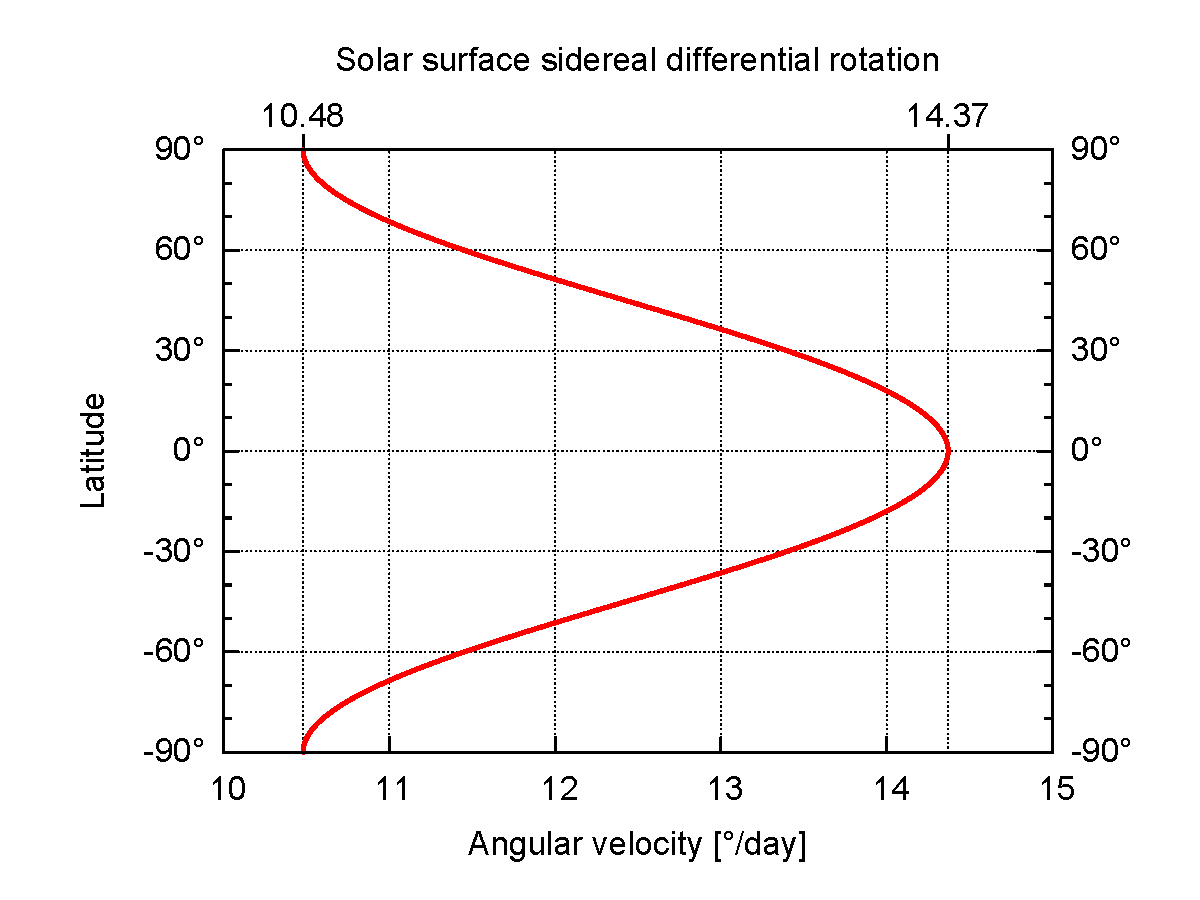
\includegraphics[width=0.5\textwidth]{images/gnuplots/differential_rotation_pdfcairo_plot.pdf}
	}{
		\caption{Diagram of the sidereal solar surface differential rotation. It shows the angular velocity for different latitudes. remove sides...}
		\label{fig:differential_rotation_pdfcairo_plot}
	}
\end{figure}

\noindent Thus, the solar equatorial rotation period (sidereal) is
\begin{align}
	T_\odot^\text{eq} &= 360\degree / A\\
	&= 25.05~\text{d}	\nonumber\\
\shortintertext{and the synodic period is}
	T_\odot^\text{eq,syn} &= 1/(1/T_\odot^\text{eq} - 1/T_\text{Earth})\\
	&= 26.90~\text{d}	\nonumber
\end{align}
with the Earth's orbital rotation period $T_\text{Earth} = 365.25$~d (1/100 Julian century).\\

Solar surface rotation period at equator\\
sidereal: 25.05~d (Sun Fact Sheet...), synodic: 26.90~d (derived)\\
Solar surface rotation period at poles:\\
sidereal: 34.35~d (diff. rot. formula), synodic: 37.92~d (derived)\\
are listed in \autoref{tab:solar_surface_rotation_periods}.\\
\begin{table}[htb]\small
	\centering
	\captionsetup{belowskip=4pt}
	\caption{Solar surface rotation periods for equator, \SI{+-16}{\degree}~latitude and poles (sidereal and synodic).}
	\begin{tabular}{llll}
		\toprule
				&Equator	&\SI{+-16}{\degree}~latitude	&Poles\\
				&\multicolumn{1}{c}{[d]}	&\multicolumn{1}{c}{[d]}	&\multicolumn{1}{c}{[d]}\\
		\midrule
		Sidereal	&25.05	&25.38	&34.35\\
		Synodic	&26.90	&27.2753$^\text{a}$	&37.92\\
		\bottomrule
		\multicolumn{4}{l}{\footnotesize{$^\text{a}$Carrington solar rotation period}}
	\end{tabular}
	\label{tab:solar_surface_rotation_periods}
\end{table}


%meridional flow

The meridional circulation is the proposed equatorial updrift and polar downdrift - a result of Reynolds stress and convective transport (cite?).\\


\section{Earth orbit geometry}

%all from https://en.wikipedia.org/wiki/Earth's_orbit
%see also http://nssdc.gsfc.nasa.gov/planetary/factsheet/earthfact.html
orbit defines ecliptic\\

Earth orbit parameters (cite?):\\
semimajor axis: $a = 1.000001018$~au\\
eccentricity: $e = 0.0167086$~au\\
%perihelion, point on solar orbit with minimum distance to Sun\\
%aphelion, point on solar orbit with maximum distance to Sun\\
distance at perihelion: (formula cite?, accuracy?)\\
\begin{align}
	r_\text{p} &= a (1 - e)\\
		&= 0.98329~\text{au}	\nonumber
\end{align}
distance at aphelion:\\
\begin{align}
	r_\text{p} &= a (1 + e)\\
		&= 1.0167~\text{au}	\nonumber
\end{align}

for calculation of heliospheric distance see HORIZONS Web-Interface at \url{http://ssd.jpl.nasa.gov/horizons.cgi}

perihelion/aphelion times...
%http://aa.usno.navy.mil/data/docs/EarthSeasons.php

\subsection{Solar distance}

Sun-Earth distance over the course of the year.\\
In the year 2017 Earth's perihelion was on 5~January with a distance of \SI{-1.67}{\percent} from \SI{1}{\au} (Horizons On-Line Ephemeris System\footnote{\url{http://ssd.jpl.nasa.gov/horizons.cgi}}, Solar System Dynamics Group, Jet~Propulsion Laboratory).\\
The cosine approximation
\begin{align}
	r_\text{E}(t) = 1 - 0.0167 \cdot \cos\left(2 \pi \left(t - 2017 - \frac{5}{365}\right)\right)\,,
\end{align}
with $t$ in years, suffices for our accuracy requirements.\\
% HORIZONS Web-Interface
% http://ssd.jpl.nasa.gov/horizons.cgi
% Ephemeris Type:	VECTORS
% Target Body:		Earth [Geocenter] [399]
% Coordinate Origin:	Sun (body center) [500@10]
% Time Span:		Start=2017-01-01, Stop=2017-12-31, Step=1 d
% Table Settings:	CSV format=YES
% Display/Output:	download/save (plain text file)
%-> distance:	9.833098226363186E-01
%-> diff. to 1 au:	0.166901774
%-> change to day before:	4.4e-6	-> 0.1669018(44)

seasonal variation function:\\
$X_\text{avg}(t) = a\,r_\text{E}(t)^b$\\
% B_avg = 5.969(29)~nT\\
% B_med = 5.435(24)~nT\\
% N_avg = 6.329(85)~cm-3\\
% N_med = 4.858(60)~cm-3\\
% T_avg = 1.198(16)e5~K\\
% T_med = 7.17(12)e4~K\\
% V1_avg = 4.132(22)e2~km/s\\
% V1_med = 4.034(21)e2~km/s\\
% V2_avg = 4.132(22)e2~km/s\\
% V2_med = 4.034(21)e2~km/s\\

\subsection{Solar rotation axis tilt}
%\label{sec:}

The inclination of the solar equator to the ecliptic (tilt/obliquity) is $i_\odot = 7.25$\textdegree{} \citep{USNO2015}. %C3

Viewed from Earth the projected solar rotation axis tilt angle varies as the Earth is moving on its orbit.\\

At the time XX the angle is zero.\\

The projected tilt angle to Earth over the year is\\

% Stonyhurst disk
% 
% Calculation of solar tilt angle at given time
% solar tilt/obliquity to ecliptic: i_sun = 7.25\degrees (Sun fact sheet: \url{http://nssdc.gsfc.nasa.gov/planetary/factsheet/sunfact.html)}
% modulate this angle with a sine over the year:
% projected tilt from Earth: i_proj = i_sun * sin(beta)
% this years vernal equinox: eq = 2015.0 + 2.0/12.0 + 20.0/365.0 = 2015.2215
% actual separation angle from vernal equinox position: phi = (today - eq) * 360
% 
% ecliptic longitude: \url{http://cohoweb.gsfc.nasa.gov/helios/plan_des.html}
% Ecliptic longitude of ascending node of the Sun's equator
% http://sspg1.bnsc.rl.ac.uk/SEG/Coordinates/angles.htm

%Hapgood (1992), Space Physics Coordinate Transformations: A User Guide
\citet{Hapgood1992}:
\begin{align}
	\omega = 73.67 + 0.013\,958 * (today - 1850.0)	%#why? yearly change
\end{align}
% beta = phi - omega
% 
% Meridians (longitude lines)
% 
% Parallels (latitude lines)


% vernal_equinox = 2016.0 + 2.0/12.0 + 20.0/366.0
% tilt(x) = 7.25 * sin(-(73.67 + 0.013958 * (x - 1850.0)) + (-vernal_equinox + x) * 360.0)
% 
% 	tilt(2016.0+(x-1.0)/12.0) with lines title "sine approx." ls 2 lw 2,\

solar tilt over the year, see \autoref{fig:Solar_tilt_seasons_plot}
\begin{figure}[htb]
	%\centering
	\fcapside[\FBwidth]{
		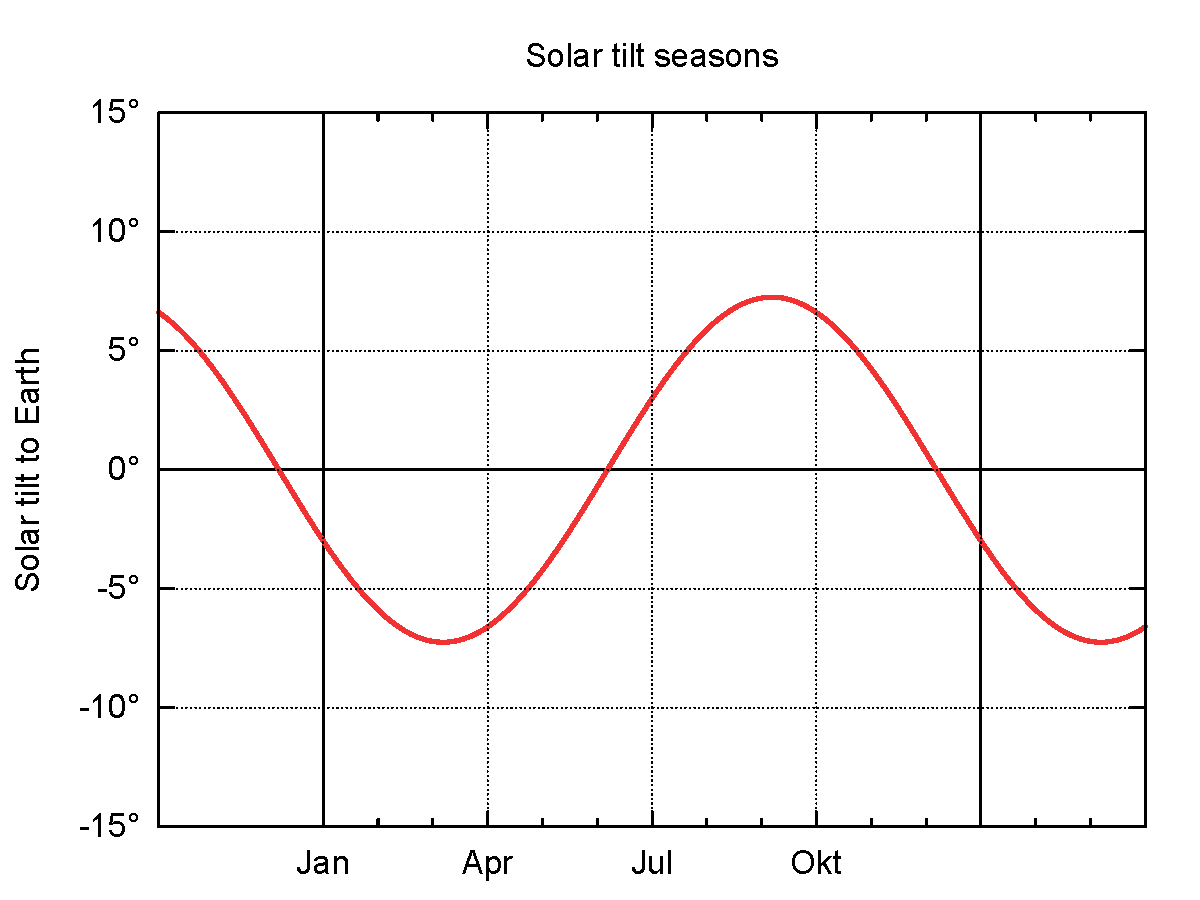
\includegraphics[width=0.5\textwidth]{images/gnuplots/Solar_tilt_seasons_plot.pdf}
	}{
		\caption{Projected solar tilt angle over the year as viewed from Earth. remove sides...}
		\label{fig:Solar_tilt_seasons_plot}
	}
\end{figure}

\subsection{Earth tilt}


\section{Coordinate systems}
\label{sec:coordinate_systems}

Coordinate systems used in this thesis:\\
GSE - Geocentric Solar Ecliptic\\
GSM - Geocentric Solar Magnetospheric\\
%RTN - Radial Tangential Normal\\
%SE - Solar Ecliptic\\
%SSE - Sun-centered Solar Ecliptic\\
HGI - Heliographic Inertial\\

refer to \citet{Hapgood1992} for GSE and GSM\\

figures for GSE and GSM

% RTN - Radial Tangential Normal
%     Spacecraft centered coordinate system. 
%     R = Sun to Spacecraft unit vector 
%     T = (Omega x R) / | (Omega x R) |
%         where Omega is Sun's spin axis (in J2000 GCI)
%     N completes the right-handed triad

%R is a unit vector pointing from the Sun to the spacecraft. T is Omega x R, where Omega is a unit vector along the Sun's rotation axis. N = R x T.

% The RTN system is fixed at a spacecraft (or the planet). The R axis is directed
% radially away from the Sun, the T axis is the cross product of the solar
% rotation axis and the R axis, and the N axis is the cross product of R and T. 
% At zero Heliographic Latitude when the spacecraft is in the solar equatorial
% plane the N and solar rotation axes are parallel.
%source: http://cdaweb.gsfc.nasa.gov/misc/NotesU.html#UY_COHO1HR_MERGED_MAG_PLASMA
  
%http://omniweb.sci.gsfc.nasa.gov/coho/helios/plan_des.html
%Solar Ecliptic Coordinate System (SE)
%The SE is a heliocentric coordinate system with the Z-axis normal to and northward from the ecliptic plane. The X-axis extends toward the first point of Aries (Vernal Equinox, i.e. to the Sun from Earth in the first day of Spring). The Y-axis completes the right handed set. The Vernal Equinox direction changes slowly; commonly invoked equinox epochs are (1) B-1950, (2) Mean-of-(current) Date, and (3) J-2000. The ecliptic longitude SE_LONG increases from zero in the x-direction towards Y-direction; the latitude, SE_LAT increases to +90 deg towards north ecliptic pole and to -90 deg towards south pole.These Lat/Long are designated as ELAT and ELON in output.

%SSE - Sun-centered Solar Ecliptic coordinates

%HGI - Heliographic Inertial coordinates
%The HGI coordinates are Sun-centered and inertially fixed with respect to an X-axis directed along the intersection line of the ecliptic and solar equatorial planes, and defines zero of the longitude, HGI_LONG. The solar equator plane is inclined at 7.25 degrees from the ecliptic. This direction was towards ecliptic longitude of 74.367 deg on 1 January 1900 at 12:00 UT; because of the precession of the Earth's equator, this longitude increases by 1.4 deg/century. The Z-axis is directed perpendicular to and northward of the solar equator, and the Y-axis completes the right-handed set. The longitude, HGI_LONG increase from zero in the X-direction towards Y-direction.The latitude HG_LAT increases to +90 deg towards the north pole, and to -90 deg towards south pole.These Lat/Long are designated as HLAT & HILON in output

% The Heliographic Inertial (HGI) coordinates are Sun-centered and inertially
% fixed with respect to an X-axis directed along the intersection line of the
% ecliptic and solar equatorial  planes. The solar equator plane is inclined at
% 7.25 degrees from the ecliptic. This direction was towards ecliptic longitude of
% 74.36 degrees  on  1  January  1900  at  1200  UT; because of precession of the
% celestial equator, this longitude increases by 1.4 degrees/century. The Z axis
% is directed perpendicular and northward from the solar equator, and the Y-axis
% completes the right-handed set. This system differs from the usual heliographic
% coordinates (e.g. Carrington longitudes) which are fixed in the frame of the
% rotating Sun.
%source: http://cdaweb.gsfc.nasa.gov/misc/NotesU.html#UY_COHO1HR_MERGED_MAG_PLASMA


\subsection{Geocentric Solar Ecliptic}
\label{sec:geocentric_solar_ecliptic}

The Geocentric Solar Ecliptic (GSE) coordinates are\\
GSE - Geocentric Solar Ecliptic\\
    X = Earth-Sun Line\\
    Z = Ecliptic North Pole

GSE coordinates are used in ACE solar wind data, etc.

%http://www.srl.caltech.edu/ACE/ASC/coordinate_systems.html
%https://www.spenvis.oma.be/help/background/coortran/coortran.html
%http://adsabs.harvard.edu/abs/1992P%26SS...40..711H


\subsection{Geocentric Solar Magnetospheric}

GSM - Geocentric Solar Magnetospheric\\
X = Earth-Sun Line\\
Z = Projection of dipole axis on GSE YZ plane\\
%(Z-axis (positive) is perpendicular to the X-axis and parallel to the projection of the negative dipole moment on a plane perpendicular to the X-axis (the northern magnetic pole is in the same hemisphere as the tail of the magnetic moment vector).)\\

GSM is defined with a time dependent dipole axis.\\
the dipole axis orientation changes over time; at 1995 the northern pole was at $l = 288.59\degree$ and $b = 79.30\degree$; more recent year (2015)?... cite?\\
% https://www.spenvis.oma.be/help/background/coortran/coortran.html#MAG

\subsection{Heliographic Inertial}

Heliographic Inertial (HGI) coordinates\\
HGI coordinates are Sun-centered with the z-axis directed along the solar rotation axis and directed northward of the solar equator. The solar equator plane is inclined \SI{7.25}{\degree} from the ecliptic.\\

HGI coordinates; latitude range \SI{-7.25}{\degree}~to~\SI{-7.25}{\degree}\\
latitude variation (see Schwenn1990, p.~127)\\
